
\documentclass{article}
\usepackage{amsmath, amsfonts, amssymb, amsthm} %packages for math-related
\usepackage[margin=1.2in]{geometry}
\usepackage[shortlabels]{enumitem}
\usepackage[utf8]{inputenc}
\usepackage{graphicx} % package for inserting images
\usepackage{commath} % package for things like \del, \cbr, and \sbr. These handle parentheses well.
\usepackage[mathscr]{euscript}%for \scr command 
\usepackage{../commands} %package with all of the commands for this class
\usepackage{url}
\setlength{\parindent}{0em} % so paragraphs aren't indented
\newcommand{\lcm}{\text{lcm}}
\newcommand{\Hom}{\text{Hom}}
\newcommand{\Ann}{\text{Ann}}
\newcommand{\Cc}{{C_c^\infty(\RR)}}
% ********************************************************** %
%               THINGS TO EDIT BELOW THIS LINE               %
% ********************************************************** %
\newcommand{\D}{\nabla}
\renewcommand{\d}{\partial}
\usepackage{wrapfig}
\title{\textsc{MATH 173 Problem Set 6}}
\author{Stepan (Styopa) Zharkov}
\date{May 11, 2022}
\begin{document}
\maketitle
\problem{1} 
 \tri
\hop 
\solution
\begin{enumerate}[(a)]
    \item This problem is straightforward. 
    \begin{align*}
        \ol{\F(\phi)(y)} &= \ol {\int_\Rn e^{-ix \cdot y}\phi(x)dx} \\
        &= \int_\Rn \ol {e^{-ix \cdot y}\phi(x)}dx \\
        &= \int_\Rn e^{ix \cdot y}\ol{\phi(x)}dx \\
        &= (2\pi)^n(2\pi)^{-n}\int_\Rn e^{ix \cdot y}\ol{\phi(x)}dx \\
        &= (2\pi)^n\F\inv\ol{\phi}(y) 
    \end{align*}
    This is what we wanted to show. \qed 
    \item We know the Fourier inversion formula holds for Schwartz functions. By part (a) and the equation about interchanging fourier transform under the integral that we saw in class, we know 
    \begin{align*}
        (2\pi)^{-n}\int_\Rn \hat{\phi}\bar{\hat{\psi}} &= \int_\Rn \hat{\phi}\check{\bar{\psi}}  \\
        (2\pi)^{-n}\int_\Rn \hat{\phi}\bar{\hat{\psi}} &= \int_\Rn \check{\hat{\phi}}\hat{\check{\bar{\psi}}}  \\
        (2\pi)^{-n}\int_\Rn \hat{\phi}\bar{\hat{\psi}} &= \int_\Rn \phi\bar{\psi}.
    \end{align*}
    Setting $\psi = \phi$, we see that 
    \begin{align*}
        \int_\Rn \abs{\hat{\phi}}^2 = (2\pi)^2\int_\Rn \abs{{\phi}}^2,
    \end{align*}
    as we wanted. \qed
\end{enumerate}

\begin{center}
    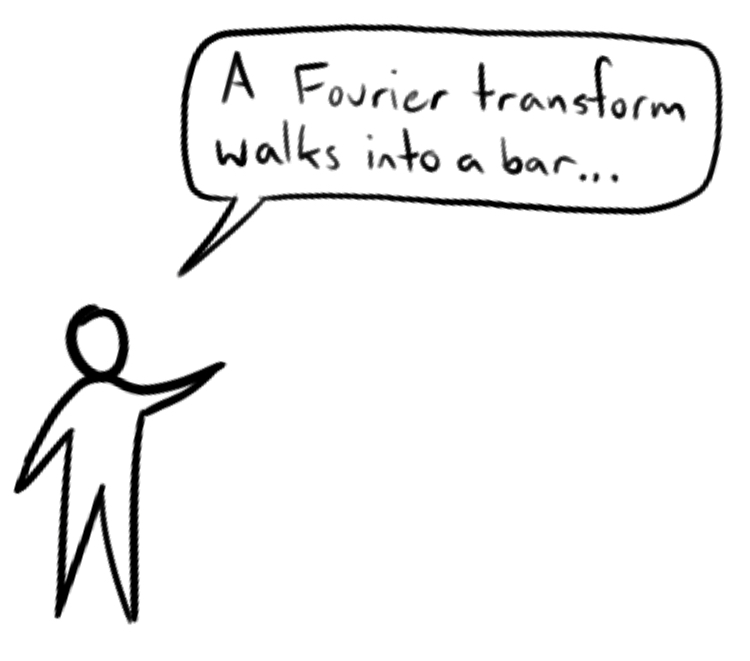
\includegraphics[height=2cm]{../images/fbar}
\end{center}

\newpage
\problem{2} 
 \tri
\hop 
\solution
\newcommand{\tu}{\tilde{u}}
\begin{enumerate}[(a)]
    \item Let $\tilde{u}(t,x)$ be defined as in the problem. On $(0, +\infty) \times (0, +\infty)$, $\tilde{u}$ is the same as $u$, so it satisfies the equation $\tu_t = \tu_{xx}$. On $(0, +\infty) \times (-\infty, 0)$, we see that 
    \[\tu_t(t,x) = -u_t(t, -x) = -u_{xx}(t, -x) = \tu_{xx}(t,x).\]
    So, $\tu_t = \tu_{xx}$ on all of  $(0, +\infty) \times (0, +\infty)  \cup (0, +\infty) \times (-\infty, 0)$ and is $C^2$ there. Now, consider the points along $x=0$. We can define $\tu(t,0)= 0$. We see that 
    \[\lim_{x \to 0} u(t,x) = u(t,0) = 0,\]
    and thus $\lim_{x \to 0} \tu(t,x) = 0$ from both sides, and is equal to $\tu(t,0)$. So, $\tu$ is continuous in $[0,+\infty)\times \RR$. 
    \hop 
    Now, let's consider differentiability. Let $t > 0$. We see that 
    \begin{align*}
        \lim_{h\to^+ 0} \frac{\tu(t,h)- \tu(t,0)}{h} &=  \lim_{h\to^+ 0} \frac{\tu(t,h)}{h} \\
        &= \lim_{h\to^+ 0} \frac{u(t,h)}{h}\\
        &= \lim_{h\to^- 0} \frac{u(t,-h)}{-h}\\
        &= \lim_{h\to^- 0} \frac{\tu(t,h)}{h}.\\
    \end{align*}
    Thus, the derivative from both sides matches up. We see that $\tu_t(t,0) = 0$. Since $u$ is continuously differentiable on the border, both components of the derivative are continuous, so $\tu$ is differentiable on $(0, +\infty) \times \RR$. 
    \hop 
    We can now assume that $\tu = K_t * \tilde{g}$. Writing this out, we have 
    \begin{align*}
        \tu(t,x) &= (K_t * \tilde{g})(x)\\
        &= \int(4\pi t)^{-1/2} e^{-\frac{|x-y|^2}{4t}} \tilde{g}(y)dy\\
        &=  \frac{1}{\sqrt{4\pi t}}\int_{0}^\infty  e^{-\frac{|x-y|^2}{4t}} \tilde{g}(y)dy+ \frac{1}{\sqrt{4\pi t}}\int_{-\infty}^0  e^{-\frac{|x-y|^2}{4t}} \tilde{g}(y)dy\\
        &=  \frac{1}{\sqrt{4\pi t}}\int_{0}^\infty  e^{-\frac{(x-y)^2}{4t}} g(y)dy- \frac{1}{\sqrt{4\pi t}}\int_{0}^\infty  e^{-\frac{(x+y)^2}{4t}} g(y)dy\\
        &=  \frac{1}{\sqrt{4\pi t}}\int_{0}^\infty  g(y)\del{ e^{-\frac{(x-y)^2}{4t}} - e^{-\frac{(x+y)^2}{4t}}}dy.\\
    \end{align*} 
    Restricting to to half, we see that 
    \[u(t,x) = \frac{1}{\sqrt{4\pi t}}\int_{0}^\infty  g(y)\del{ e^{-\frac{(x-y)^2}{4t}} - e^{-\frac{(x+y)^2}{4t}}}dy.\]
    We can verify that the boundary conditions match. \qed
    \item This is very similar to part (a), but this time let us define 
    \[\tu(t,x) = \begin{cases}
        u(t,x) &\text{ if } x \ge 0 \\
        u(t,-x) &\text{ if } x \ge 0 \\
    \end{cases}\]
    to be the even extension. 
    \hop 
    We know $\tu$ is $C^2$ and satisfies the equation on  $(0, +\infty) \times (0, +\infty)  \cup (0, +\infty) \times (-\infty, 0)$ for the same reason as in part (a). 
    \hop 
    We see that 
    \[\lim_{x \to 0} u(t,x) = u(t,0),\]
    and thus $\lim_{x \to 0} \tu(t,x) = u(t,0)$ from both sides, and is equal to $\tu(t,0)$. So, $\tu$ is continuous in $[0,+\infty)\times \RR$. 
    \hop 
    Now, we notice that 
    \begin{align*}
        \lim_{h\to^+ 0} \frac{\tu(t,h)- \tu(t,0)}{h}
        &= \lim_{h\to^+ 0} \frac{u(t,h) - u(t,0)}{h}\\
        &= 0 \\
        &= \lim_{h\to^+ 0} -\frac{u(t,h) - u(t,0)}{h}\\
        &= \lim_{h\to^- 0} -\frac{u(t,-h) - u(t,0)}{h}\\
        &= \lim_{h\to^- 0} \frac{\tu(t,h)-\tu(t,0)}{h}.\\
    \end{align*}
    Thus, the derivative from both sides matches up. We see that $\tu_t(t,0) = 0$. Since $u$ is continuously differentiable on the border, both components of the derivative are continuous, so $\tu$ is differentiable on $(0, +\infty) \times \RR$. 
    \hop 
    Making a similar assumption, we see that this time 
    \begin{align*}
        \tu(t,x) &= (K_t * \tilde{g})(x)\\
        &= \int(4\pi t)^{-1/2} e^{-\frac{|x-y|^2}{4t}} \tilde{g}(y)dy\\
        &=  \frac{1}{\sqrt{4\pi t}}\int_{0}^\infty  e^{-\frac{|x-y|^2}{4t}} \tilde{g}(y)dy+ \frac{1}{\sqrt{4\pi t}}\int_{-\infty}^0  e^{-\frac{|x-y|^2}{4t}} \tilde{g}(y)dy\\
        &=  \frac{1}{\sqrt{4\pi t}}\int_{0}^\infty  e^{-\frac{(x-y)^2}{4t}} g(y)dy+ \frac{1}{\sqrt{4\pi t}}\int_{0}^\infty  e^{-\frac{(x+y)^2}{4t}} g(y)dy\\
        &=  \frac{1}{\sqrt{4\pi t}}\int_{0}^\infty  g(y)\del{ e^{-\frac{(x-y)^2}{4t}} + e^{-\frac{(x+y)^2}{4t}}}dy.\\
    \end{align*} 
    Restricting to to half, we see that 
    \[u(t,x) = \frac{1}{\sqrt{4\pi t}}\int_{0}^\infty  g(y)\del{ e^{-\frac{(x-y)^2}{4t}} - e^{-\frac{(x+y)^2}{4t}}}dy.\]
    We can verify that the boundary condition matches. \qed
\end{enumerate}


\newpage
\problem{3} 
 \tri
\hop 
\solution
This problem is full of tricks and surprises. First, consider $v(t,x) = u(t,x) - a(t)$. This means that 
\[v_t = u_t - a'(t) = u_{xx} - a'(t)= v_xx - a'(t).\]
So, 
\[v_t - v_{xx} = -a'(t)\]
with $v(t,0)= 0$ and $v(0,x) = 0$. Also, $a(0)= 0$. So, we have an inhomogeneous heat equation.
\hop 
Let $S_t(\phi)$ be the operator in problem 2. More precisely, let 
\[S_t(\phi)(x) = \frac{1}{\sqrt{4\pi t}} \int_0^\infty \phi(y)\del{e^{-\frac{(x-y)^2}{4t}} - e^{-\frac{(x+y)^2}{4t}}}dy.\] 
Then, by Duhamel's principle, 
\[v(t,x) = \int_0^tS_{t-s}(f(s, \cdot))ds\]
where $f(t,x) = -a'(t)$. Expanding, and changing variables, we have 
\begin{align*}
    v(t,x) &= \int_0^t \frac{1}{\sqrt{4\pi (t-s)}} \int_0^\infty -a'(s)\del{e^{-\frac{(x-y)^2}{4(t-s)}} - e^{-\frac{(x+y)^2}{4(t-s)}}}dy ds \\
    &= \int_0^t \frac{-a'(s)}{\sqrt{4\pi (t-s)}} \sbr{\int_0^x e^{-\frac{(y)^2}{4(t-s)}}dy+\int_0^\infty e^{-\frac{(y)^2}{4(t-s)}}dy-\int_x^\infty e^{-\frac{(y)^2}{4(t-s)}}dy} ds\\
    &= \int_0^t \frac{-a'(s)}{\sqrt{4\pi (t-s)}} \sbr{\int_0^x e^{-\frac{(y)^2}{4(t-s)}}dy+\int_0^x e^{-\frac{(y)^2}{4(t-s)}}dy} ds\\
    &= \int_0^t \frac{-2a'(s)}{\sqrt{4\pi (t-s)}}\int_0^x e^{-\frac{(y)^2}{4(t-s)}}dy ds
\end{align*}
Now, using the hint, we can change variables and apply integration by parts to see that 
\begin{align*}
    v(t,x) &=  \int_0^t \frac{-2a'(s)}{\sqrt{\pi}}\int_0^{x(4(t-s))^{-1/2}} e^{-z^2}dz ds\\
    &= \frac{-2a(t)}{\sqrt{\pi}} \cdot \frac{\sqrt{\pi}}{2}+   \int_0^t \frac{-2a(s)}{\sqrt{\pi}} e^{\frac{-x^2}{4(t-s)}} \del{-(t-s)^{-3/2} \cdot \frac{1}{4}} ds\\
    &= - a(t)+ \frac{x}{\sqrt{4\pi}}\int_0^t (t-s)^{-3/2} e^{\frac{-x^2}{4(t-s)}}a(s) ds\\
    &=  - a(t)+\frac{x}{\sqrt{4\pi}}\int_0^t s^{-3/2} e^{\frac{-x^2}{4(s)}}a(t-s) ds.
\end{align*}
Thus, we can conclude that 
\[u(t,x)=\frac{x}{\sqrt{4\pi}}\int_0^t s^{-3/2} e^{\frac{-x^2}{4(s)}}a(t-s) ds,\]
which is what we wanted. Note that the integral is only converges for $x> 0$, so we can add on that $u(t,0) = a(t)$.  \qed
\newpage
\problem{4} 
 \tri
\hop 
\solution
\begin{enumerate}[(a)]
    \item By d'Alembert's formula, we know 
    \begin{align*}
        u(x,t) &= \frac{1}{2}(\phi(x+ct)+\phi(x-ct)) + \frac{1}{2c}\int_{x-ct}^{x+ct} \psi(\sigma) d \sigma\\
        &= \frac{1}{2}((x+ct)^2+(x-ct)^2) + \frac{1}{2c}\int_{x-ct}^{x+ct} 1 d \sigma\\
        &= x^2 + (ct)^2 + t^2.
    \end{align*}
    \qed
    \item For this problem, we can repeatedly use the fundamental theorem of calculus. We assume that $u_x$ vanishes at infinity. We see 
    \begin{align*}
        \int u(t,x) dx &= \int \del{u(0,x) + \int_0^t u_t(\tau, x)d\tau} dx \\
        &= \int \del{u(0,x) + \int_0^t \del{u_t(0, x) +\int_0^\tau u_{tt}(s,x)ds}d\tau} dx\\
        &= \int \del{u(0,x) + \int_0^t \del{u_t(0, x) +\int_0^\tau c^2u_{xx}(s,x)ds}d\tau} dx\\
        &= \int u(0,x) dx  +\int \int_0^t u_t(0, x) d\tau dx+\int \int_0^t \int_0^\tau c^2u_{xx}(s,x)dsd\tau dx\\
        &= \int \phi(x) dx  +\int \int_0^t \psi(x) d\tau dx+\int \int_0^t \int_0^\tau c^2u_{xx}(s,x)dsd\tau dx\\
        &= \int \phi(x) dx  +t\int \psi(x) d\tau dx+ \int_0^t \int_0^\tau \int c^2u_{xx}(s,x) dx dsd\tau \\
        &= \int \phi(x) dx  +t\int \psi(x) d\tau dx+ \int_0^t \int_0^\tau 0\  dsd\tau \\
        &= \int \phi(x) dx  +t\int \psi(x) d\tau dx,
    \end{align*}
    exactly as we wanted. \qed
\end{enumerate}


\newpage
\problem{5} 
 \tri
\hop 
\solution
To solve this, we take the partial Fourier transform of 
\[u_{tt} = u_{xx} - m^2u\]
to get 
\[\hat{u}_tt = -y^2 \hat{u} - m^2 \hat{u}\]
with conditions 
\[\hat{u}(0,y) = \hat{g}(y), \ \hat{u}_t(0,y) = \hat{h}(y).\]
Solving this ODE, we have that 
\[\hat{u} = \cos{\sqrt{y^2 + m^2}yt}\hat{g}(y) + \frac{\sin(\sqrt{y^2+m^2}yt)}{\sqrt{y^2+m^2}}\hat{h}(y).\]
This is the solution we were looking for. \qed

\newpage
\problem{6} 
 \tri
\hop 
\solution
The hint unlocks the secret to this problem. Suppose no such $C, m$ exist. In particular, no constant $C = m = j \in \NN$ works. Let $\phi_j \in \cal{S}(\Rn)$ be the counterexample that gives $\abs{U(\phi_j)} > j||\phi_j||_j$. Now, let's define 
\[\psi_j = j\inv||\phi_j||_j\inv\phi_j.\]
Since $\phi_j$ are Schwartz, for any multi-indices $\alpha, \beta$,  $x^\alpha \d^\beta \phi_j$ are bounded. For any $\eps > 0$, select $j > \max(\eps \inv, |\alpha| , |\beta|)$. Then, 
\begin{align*}
    \sup_x\abs{x^\alpha \d^\beta \psi_j} &= \sup_x \abs{x^\alpha \d^\beta j\inv \del{\sum_{|{\sf{a}}|, |{\sf{b}}| < j} \sup_{y} \abs{y^{\sf a} \d^{\sf b} \phi_j(y)}}\inv \phi_j(x)}\\
    &= j\inv \frac{ \sup_x \abs{x^\alpha \d^\beta \inv \phi_j(x)}}{\sum_{|{\sf{a}}|, |{\sf{b}}| < j} \sup_{y} \abs{y^{\sf a} \d^{\sf b} \phi_j(y)}} \\
    &\le j\inv \\
    &< \eps.
\end{align*}
Thus, by definition, $\psi_j \to 0$ as a Schwartz function. 
\hop 
However, we see that by linearity of $U$, 
\begin{align*}
    \abs{U(\psi_j)} &= \abs{U(j\inv||\phi_j||_j\inv\phi_j)}\\
    &= \abs{U(\phi_j)}j\inv||\phi_j||_j\inv \\
    &> 1
\end{align*}
by our choice of $\phi_j$. But $U(0)=0$, so $U$ is not continuous and we have a contradiction. Thus, 
the constants $C$ and $m$ must exist. \qed 


\newpage
\problem{7} 
 \tri
\hop 
\solution
\begin{enumerate}[(a)]
    \item For this problem, we must go back to the definition of an integral through Riemann sums. First, notice that 
    \begin{align*}
        \int_\Rn g(y)\phi(y)dy &= \int_\Rn U(f(x)e^{-i x \cdot y})\phi(y) dy \\
        &= \int_\Rn U(f(x)e^{-i x \cdot y}\phi(y)) dy \\
        &= \lim_{N \to \infty} \sum^N_{k=1} |I_k| U(f(x)e^{-i x \cdot y_k}\phi(y_k))\\
        &= \lim_{N \to \infty}  U\del{\sum^N_{k=1} |I_k| f(x)e^{-i x \cdot y_k}\phi(y_k)}
    \end{align*}
    where $y_k$ is some point in the Riemann cube $I_k$ and the limit notation denotes taking smaller and smaller intervals and covering more and more of space. 
    \hop 
    We want to be able to move the integral inside of $U$, but we can't do that directly. We can move the finite sum inside by linearity of $U$, and continuity gives us that we can move the limit inside as long as the inside converges as Schwartz functions. So, let us show that 
    \[\sum^N_{k=1} |I_k|f(x)e^{-i x \cdot y_k}\phi(y_k) \to \int f(x)e^{-ix \cdot y} \phi(y)dy\]
    in the Schwartz sense. First, we know $f$ has compact support, so we can assume $x$ is bounded by some constant $R$. Let $\alpha, \beta$ be multi-indices. We need to check that 
    \[\sup_x\abs{x^\alpha \d^\beta \del{\sum^N_{k=1} |I_k|f(x)e^{-i x \cdot y_k}\phi(y_k) - \int f(x)e^{-ix \cdot y} \phi(y)dy}}\]
    converges to 0 as $N \to \infty$. When we expand out the derivatives, each term in the massive sum will be of the form 
    \[x^\alpha  \del{\sum_{k=1}^N |I_k|\d^\gamma f(x)(-iy_k)^\omega e^{-ix \cdot y_k} \phi(y_k) - \int \d^\gamma f(x) (-iy)^\omega  e^{-ix \cdot y}\phi(y) dy}\]
    where $\gamma$ and $\omega$ are some multi-indices such that $|\gamma|, |\omega| \le |\beta|$. Since $\phi$ is a Schwartz function, $(iy)^\omega \phi(y)$ is bounded. By definition of an integral, the expression inside the parentheses converges to 0 pointwise (for a set $x$). The expression is continuous and has compact support (because $\d^\gamma$ has compact support). We know that poinwise convergence of continuous functions on compact support implies uniform convergence. So, there is some sequence $M_N$ such that $M_N \to 0$ and 
    \[\sum_{k=1}^N |I_k|\d^\gamma f(x)(-iy_k)^\omega e^{-ix \cdot y_k} \phi(y_k) - \int \d^\gamma f(x) (-iy)^\omega e^{-ix \cdot y}\phi(y) dy < M_N.\]
    Thus we see that 
    \begin{align*}
        &\sup_{x} \abs{x^\alpha \del{\sum_{k=1}^N |I_k|\d^\gamma f(x)(-iy_k)^\omega e^{-ix \cdot y_k} \phi(y_k) - \int \d^\gamma f(x) (-iy)^\omega e^{-ix \cdot y}\phi(y) dy}} \\
        =&\sup_{x<R} \abs{x^\alpha \del{\sum_{k=1}^N |I_k|\d^\gamma f(x)(-iy_k)^\omega e^{-ix \cdot y_k} \phi(y_k) - \int \d^\gamma f(x) (-iy)^\omega e^{-ix \cdot y}\phi(y) dy}} \\
        \le & \sup_{x < R} \abs{x^\alpha M_N}\\
        \le & R^{|\alpha|}M_N
    \end{align*}
    This certainly converges to 0. There are only a finite number of terms like this (because there are only so many options for what derivatives to take given that $|\gamma|, |\omega| < |\beta|$). So, we can conclude that 
    \[\sup_x\abs{x^\alpha \d^\beta \del{\sum^N_{k=1} |I_k|f(x)e^{-i x \cdot y_k}\phi(y_k) - \int f(x)e^{-ix \cdot y} \phi(y)dy}} \to 0.\]
    This means that the Riemann sum does indeed converge to the integral as Schwartz functions. So, by continuity of $U$, 
    \begin{align*}
        \int_\Rn g(y)\phi(y)dy &=  \lim_{N \to \infty}  U\del{\sum^N_{k=1} |I_k| f(x)e^{-i x \cdot y_k}\phi(y_k)} \\
        &= U\del{\lim_{N \to \infty} \sum^N_{k=1} |I_k| f(x)e^{-i x \cdot y_k}\phi(y_k)} \\
        &= U\del{\int f(x)e^{-i x \cdot y}\phi(y) dy} \\
        &= U(\cal{F}(\phi)) \\
        &=\F(U)(\phi).
    \end{align*}
    With this, we are done. 
    \item Since $U$ is linear and continuous, 
    \[U(\d^\alpha f(x)e^{-ix \cdot y}) = \d^\alpha U(f(x)e^{-ix \cdot y})\]
    where the derivative is with respect to $y$ as long as $\d^\alpha f(x)e^{-ix \cdot y}$ is Schwartz in $x$. 
    \hop 
    We see that 
    \[\d^\alpha f(x)e^{-ix \cdot y}= f(x)\d^\alpha e^{ix \cdot y} = f(x)(ix)^\alpha e^{ix \cdot y}\]
    is indeed Schwartz because $f$ has compact support and is $C^\infty$. Thus, we can conclude that $g \in C^\infty$. 
    \hop 
    To show the second part, we use problem 6. We know there exist $C_0, m$ such that $|U(\phi)| \le C_0||\phi||_{m}$ for all $\phi$. This means that 
    \begin{align*}
        |g(y)| &= |U(f(x)e^{-ix \cdot y})| \\
        & \le C_0 || f(x)e^{ix \cdot y}||_{m} \\
        &= C_0 \sum_{|\alpha|,|\beta| < m}\sup_x \abs{x^\alpha \d^\beta f(x)e^{ix \cdot y}}.
    \end{align*}
    When we expand out the derivatives, each term in the sum inside the $\sup$ will be of the form 
    \[x^\alpha (iy)^\gamma e^{ix \cdot y} \d^\omega f(x)\]
    where $|\omega|, |\gamma| < m$ Since $f$ has compact support, this is only nonzero for $x < R$ for some constant $R > 1$. Also, this means each derivative of $f$ is bounded. Let $F$ be a constant that bounds all derivatives of $f$ up to $m$. Thus, 
    \begin{align*}
        \abs{x^\alpha (iy)^\gamma e^{ix \cdot y} \d^\omega f(x)} &\le R^m \abs{ (iy)^\gamma e^{ix \cdot y} \d^\omega f(x)}\\
        &\le R^m \abs{ (iy)^\gamma\d^\omega f(x)}\\
        &\le R^m F \abs{ (iy)^\gamma}\\
        &\le R^m F (\abs{y}+1)^m.
    \end{align*}
    Now, there is a finite number of terms in that sup. Call that number $S$. Then, by triangle inequality,
    \[\sup_x \abs{x^\alpha \d^\beta f(x)e^{ix \cdot y}} \le S R^m F (\abs{y}+1)^m.\]
    There are also finitely many options for $\alpha, \beta$. Call the number of options $M$. Then, we see that 
    \[|g(y)| \le C_0 M S R^m F (\abs{y}+1)^m .\]
    So, letting $C = C_0 M S R^m F$, we get the desired bound. \qed
\end{enumerate}
\begin{center}
    
\includegraphics[height=3cm]{../images/suppf}
\end{center}
\end{document}